% !TEX root = ../main.tex

\section{Problem analysis and design} \label{sec:analysis-design} 

The main challenges are already hinted at in section~\ref{sec:goals}. All these
goals pose different problems. These problems (and especially their solutions)
is best analyzed when also discussing the chosen design.



\subsection{The Basic, Simple Algorithm} \label{sec:basic-algorithm}

This building blocks for the basic, simple algorithm is this: An individual $X$
is represented as a string with the same length as the time series $Y$ with
length $T$, $|X| = T$, and $Y$ itself is represented as an array of $T$
observations. The data structures themselves are very simple. 

The design of the algorithm is found in the handed out pseudo code. Thus,
discussing the implementation and functionality of this code seems redundant.
Especially given that all the procedures are explained in \cite{doerr2017a}. 

What \textit{is} interesting about this design is the generality of it: A
genetic algorithm is a very general tool. In the most simple of cases, the
individuals manipulated are simple solution strings containing 1s and 0s - or
other simple characters. The individual is thus a simple entity, and the value
of it only becomes meaningful in the context of a given problem.

In the context of finding structural break points with the rectangle fitness
method, the genome of the individuals contains two types of alleles: \texttt{0}
meaning no break point and \texttt{1} meaning a break point. Thus, the genome
has $T$ genes, where each gene can contain one of two types of alleles. 

This general and simple approach is alluring due to its simplicity. This is
especially the case within the biological narrative of the genetic algorithm: A
genome of fixed length and a small set of alleles matches the narrative. But for
this problem, where the number of breakpoints is potentially miniscule compared
to the length of the time series, there is a more efficient approach, see
section~\ref{sec:optimized-algorithm}. 



\subsection{Graphical User Interface, GUI}

For the design of the GUI, there are two key priorities: 1) Displaying the time
series with break points and 2) being able to configure algorithm parameters. 

While the implementation of displaying the graph and showing break points was incredibly tricky, see
section~\ref{sec:graph-implementation}, the design itself is fairly easy: Show a
graph and draw some rectangles/lines. The focus here is to make the graph area
take up as much of the GUI as possible. This is achieved by being able to toggle
the settings pane, see figure~\ref{fig:gui-toggle-ex}. 

\begin{figure}[h]
    \centering
    \begin{subfigure}[b]{.48\textwidth}
        \centering
        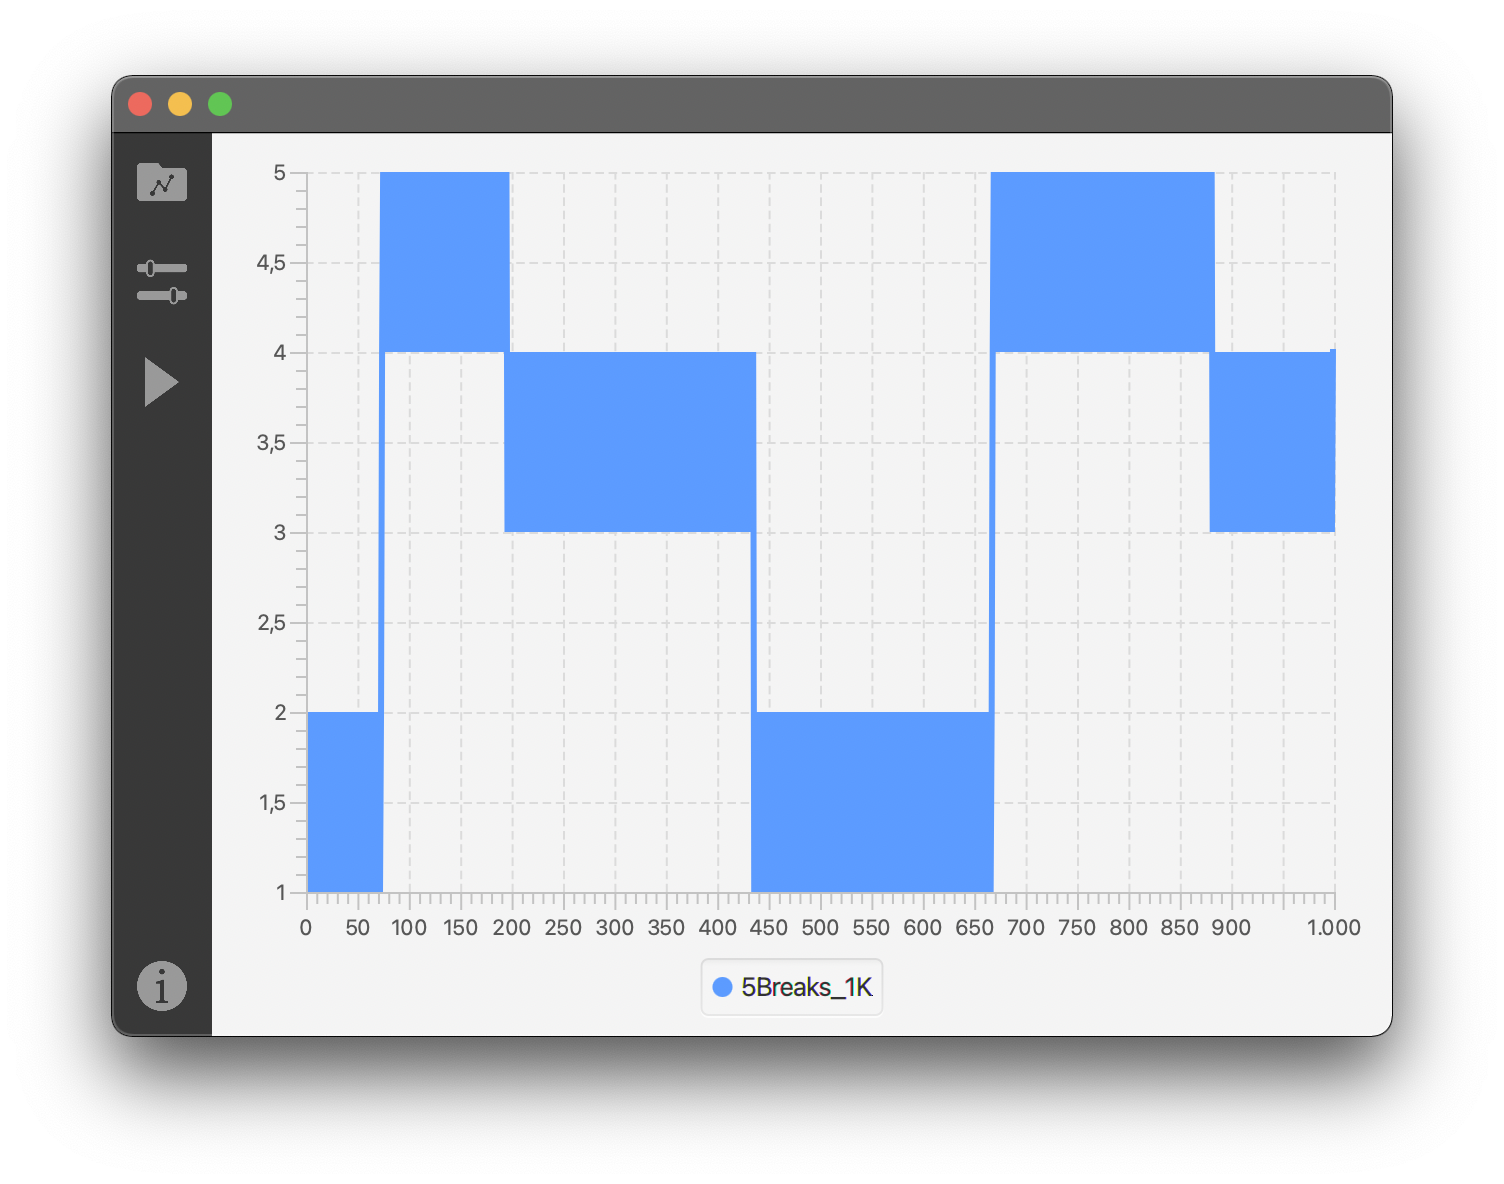
\includegraphics[width=\textwidth]{fig/gui-toggle-off.png}
        \caption{GUI not showing the settings pane}
        \label{fig:gui-toggle-off}
    \end{subfigure}
    \hfill
    \begin{subfigure}[b]{.48\textwidth}
        \centering
        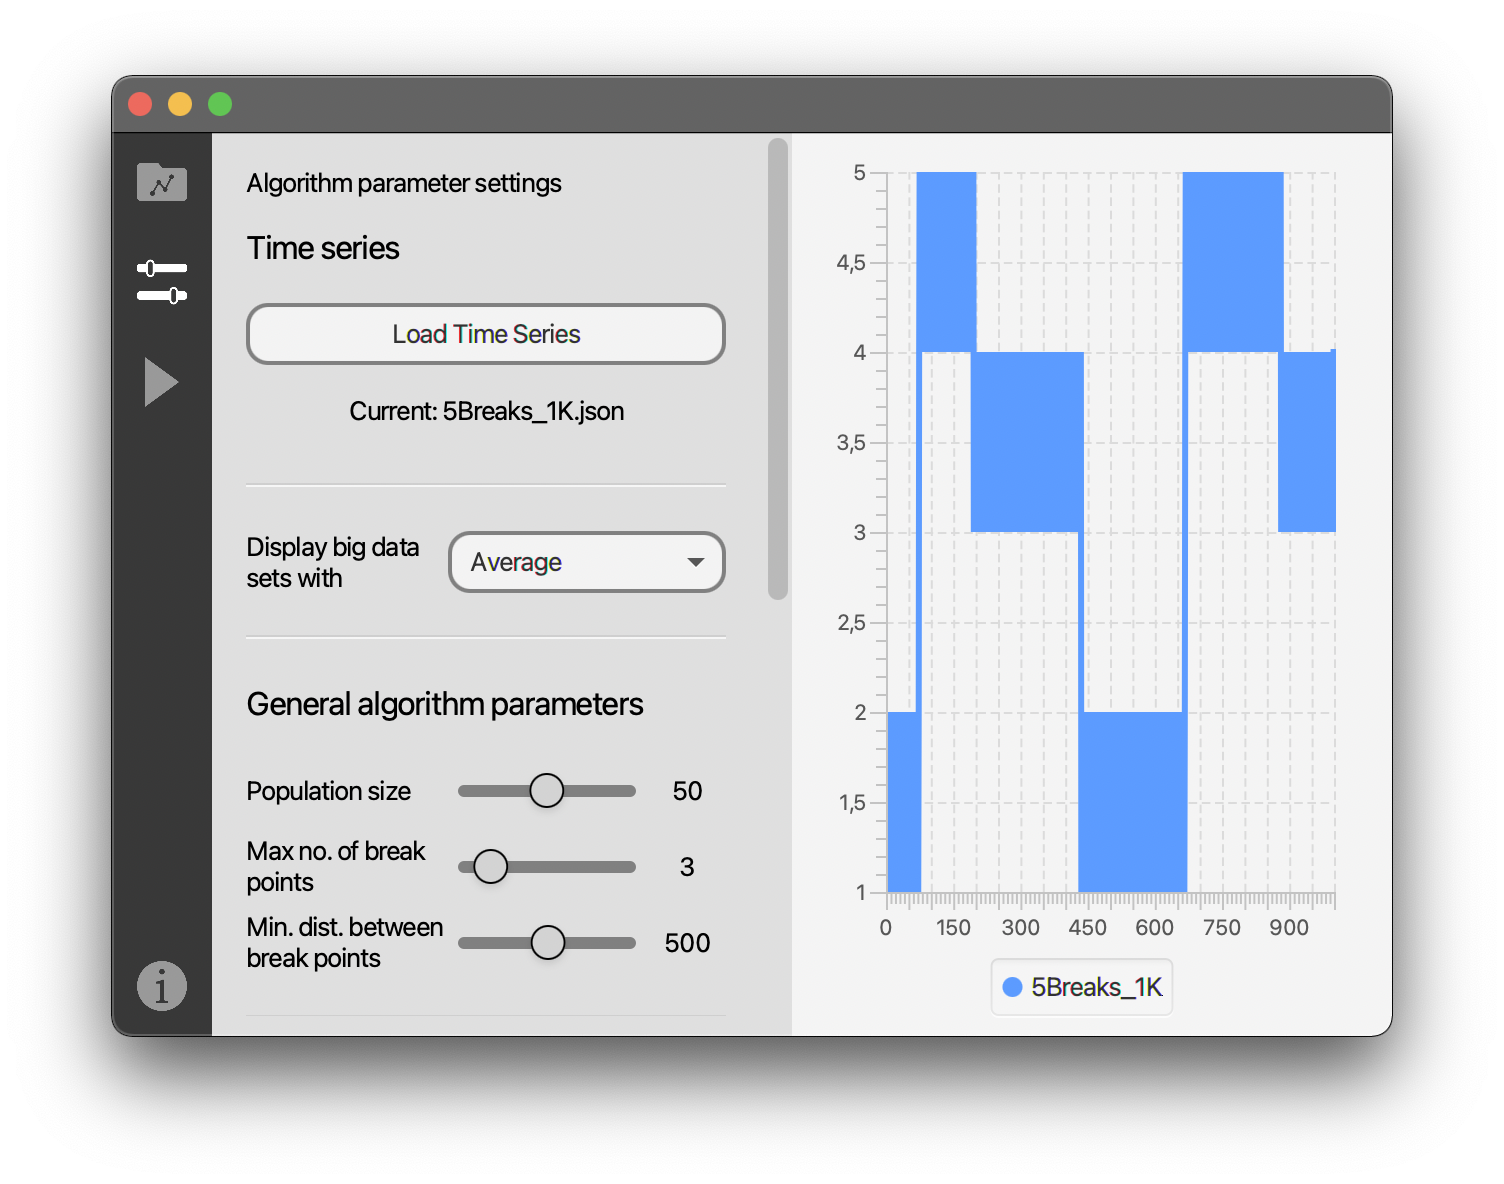
\includegraphics[width=\textwidth]{fig/gui-toggle-on.png}
        \caption{GUI showing the settings pane}
        \label{fig:gui-toggle-on}
    \end{subfigure}
    \caption{GUI with and without settings pane toggled}
    \label{fig:gui-toggle-ex}
\end{figure}

For large time series, it is unnecessary and inefficient to display all
measurements. In stead, a maximum of 1000 points are displayed on the graph. The number of
graph points per measurement $n_p$ is given by:
\begin{align}
    n_p = \left\lceil \frac{T}{1000} \right\rceil
\end{align}
Each point in the graph thus contains multiple measurements from the time
series. These multiple points can be displayed in two ways: Taking the average
of the measurements (figure~\ref{fig:gui-graph-avg}) or displaying the minimum
and maximum (figure~\ref{fig:gui-graph-min-max}). 

\begin{figure}[h]
    \centering
    \begin{subfigure}[b]{.48\textwidth}
        \centering
        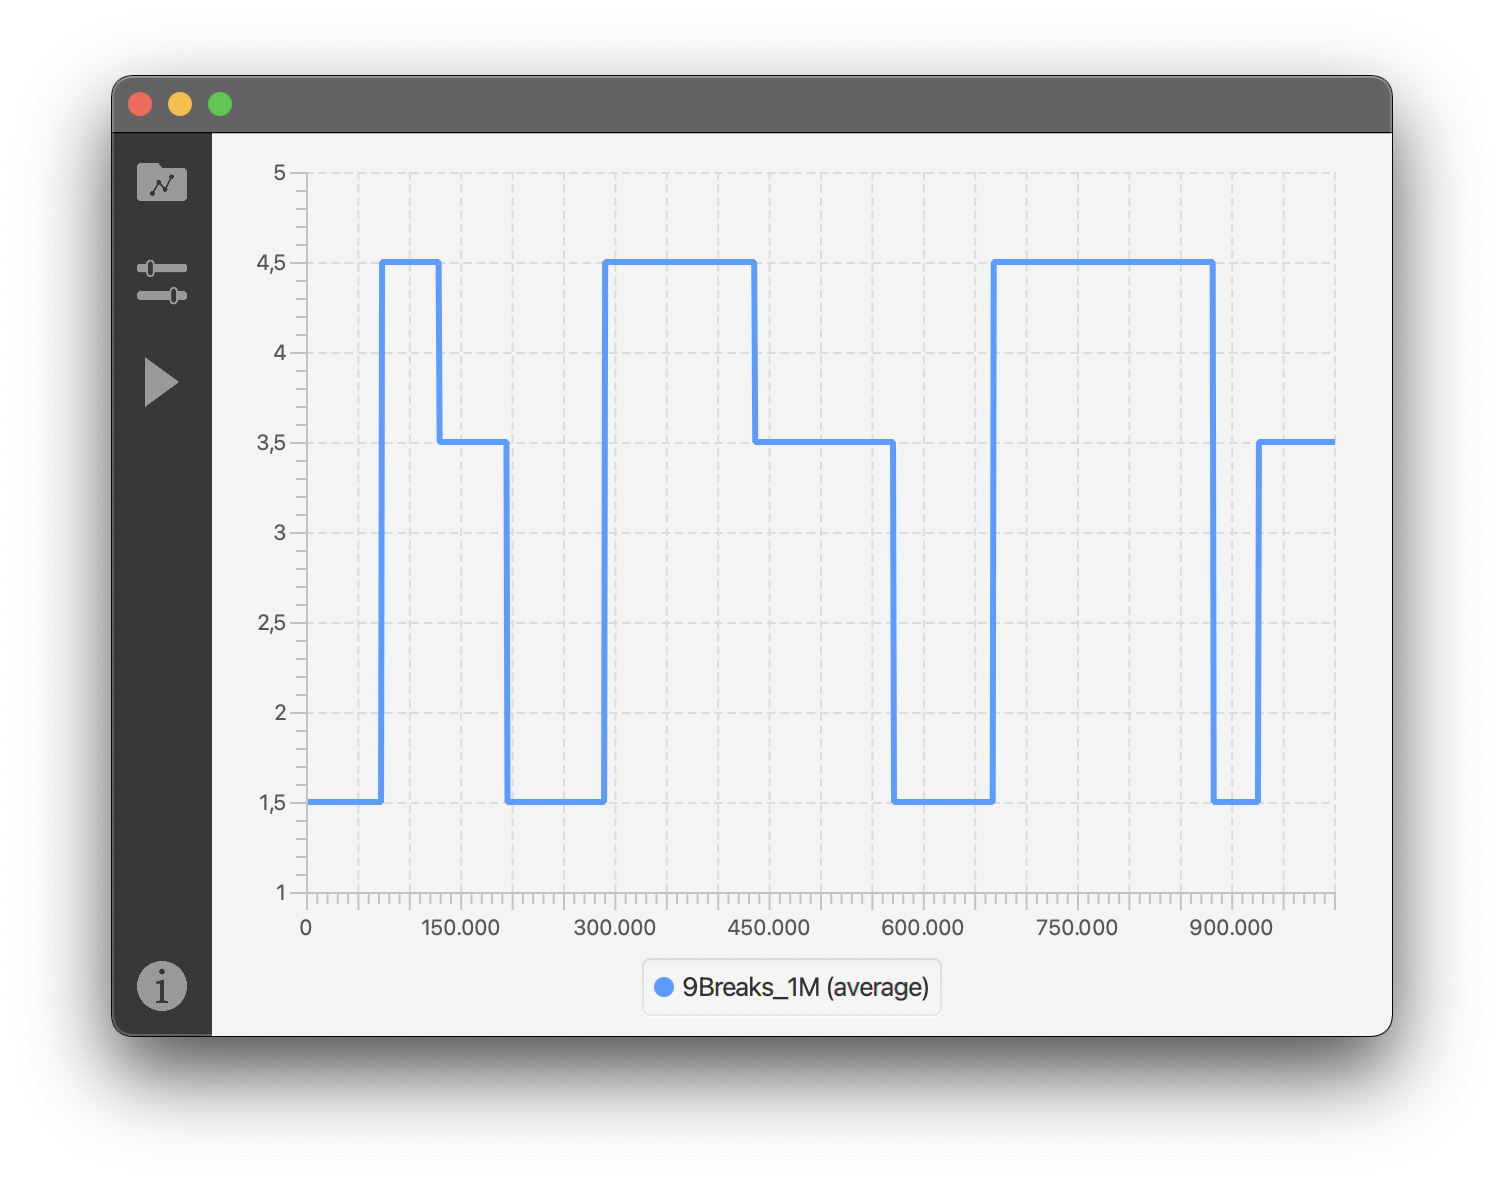
\includegraphics[width=\textwidth]{fig/gui-graph-avg.png}
        \caption{Each point on the graph is the average of 1000 observations}
        \label{fig:gui-graph-avg}
    \end{subfigure}
    \hfill
    \begin{subfigure}[b]{.48\textwidth}
        \centering
        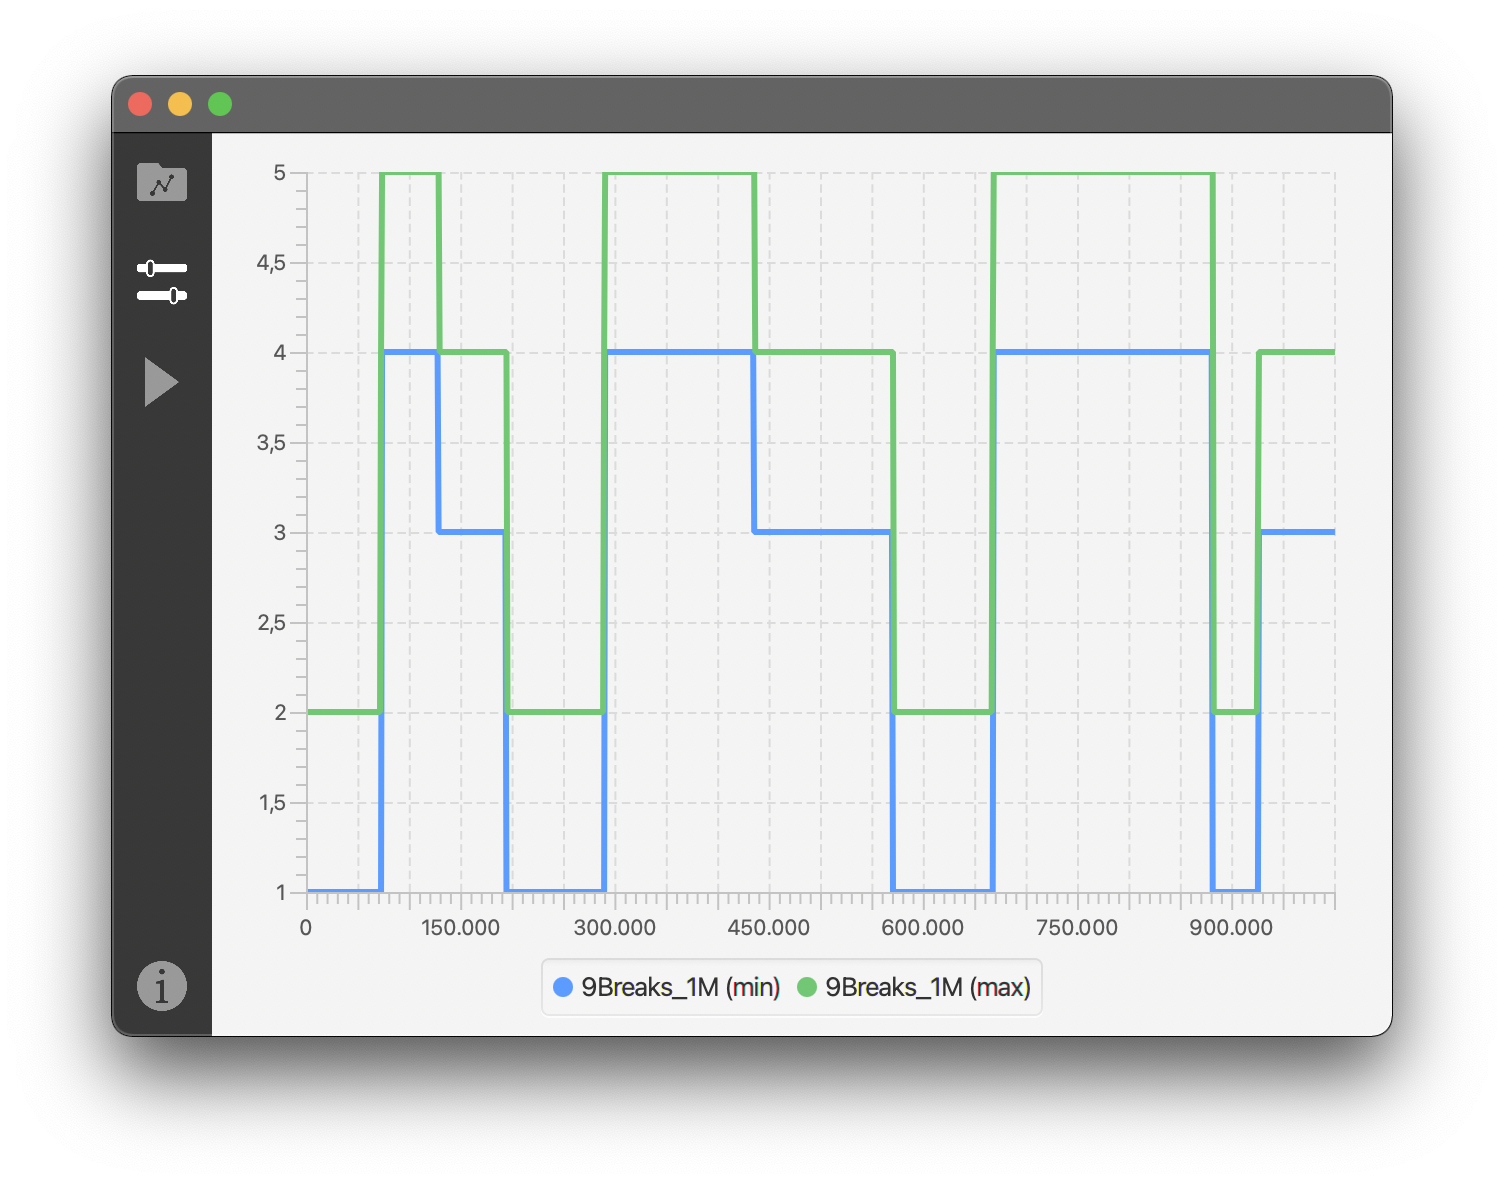
\includegraphics[width=\textwidth]{fig/gui-graph-min-max.png}
        \caption{For each 1000 observations, the min and max is displayed}
        \label{fig:gui-graph-min-max}
    \end{subfigure}
    \caption{The graph showing a time series with $T = 10^6$ observations}
    \label{fig:gui-graph-ex}
\end{figure}

For tuning the parameters, the design for this GUI has been sliders, buttons and
menus. These ways of interacting are very bulletproof as the user cannot do
anything wrong with the controls. (This is very much not the case with text
fields where a lot of error-handling is needed for even simple integer fields).
The downside to especially sliders is that they limit the user to a certain
range. The controls are reliable but not very flexible. 

A lot of the algorithm parameters can be tuned. This is definitely not all
parameters. The ones chosen go into these categories: 
\begin{description}
    \item[General algorithm parameters] Things like the size of the population,
    the maximum number of break points, and the minimum distance between the
    break points. 

    \item[Probability values] Setting the probability for each of the genetic
    algorithm procedures: mutation $p_{mu}$, one point crossover $p_{opc}$, and
    uniform crossover $p_{uc}$. Note that $p_{mu} + p_{opc} + p_{uc} = 1$. To
    solve this, the slider are connected: First, $p_{mu}$ is set, and the two
    other sliders are set to 
    \begin{align*}
        p_{opc} = p_{uc} = \frac{1 - p_{mu}}{2}
    \end{align*}
    \textit{Then} $p_{opc}$ is adjusted. When adjusting, $p_{opc} \in [0, 1 -
    p_{mu}]$ and $p_{uc} = 1 - p_{mu} - p_{opc}$. The slider for uniform
    crossover can never itself it moved, only the two other sliders can move it.
    In summation, first change the
    mutation slider, then change the one point crossover slider to dial in all
    three probabilities. 

    \item[Fitness] The user can change the fitness method (although only
    one exists now) and tune the $\alpha$-parameter for the penalty term in the
    fitness function. 
\end{description}

Besides this, the GUI can load time series data files using the system's own
file viewer and the algorithm can of course be run with the algorithm. 

\subsubsection{Model-View-Controller}

The design of the GUI is made with the Model-View-Controller pattern in mind.
The model is of course the algorithm itself. There is one entity in charge of
running the algorithm and keeping charge of the parameters. The view is simply
the look of the GUI. The placement of everything and the styling itself. Lastly,
the controller takes all inputs from the user and delivers the relevant
information to the model. 

In this case, the model is a Java class \texttt{BreakPointAlgorithm} which is
the brain of the system and the class in charge of running the algorithm itself
with all the parameters. The view is done using FXML files and styling
with CSS. Lastly, the controller is another class which communicates directly
with the model: Listeners are placed on all the controls which sends updated
parameter values to the model. 

\subsubsection{Observer pattern}

The observer pattern is only included at a small scale: The controls in the
controller have listeners that updates the model when the value is changed.
Besides that observer pattern is not implemented here as the application is very
small. A more simple approach is simply to allow the controller and the business
logic to exchange information. The business logic can, in this application,
never change if no changes are performed in the GUI. This makes observer pattern
rather useless. 


\subsection{Optimizing the algorithm} \label{sec:optimized-algorithm}

For the optimization in this project, two key areas have been optimized: 
\begin{enumerate}
    \item The genomes no longer contain genes with non-break-point-alleles. The
    genome is in stead a list-structure $G$. At each gene $g$ is an allele
    $a_g$, $G(g) = a_g = (b_g, B_g)$. The value $b_g$ is itself an index
    representing the index of the break point, $b_g \in [0, T]$. The term $B_g$
    is a more abstract value containing information relevant for the fitness
    model. 
    
    \item The time series observations are stored in a \textit{range
    tree}/\textit{interval tree}. While setting up the range tree will itself
    take longer than setting up a simple array, getting minimum and maximum
    values in index intervals is much faster. 
\end{enumerate}
Making these changes means altering the genetic algorithm procedures and
implementing the range tree data type. 



\subsubsection{Altering genetic algorithm procedures}
\label{sec:altering-procedures}

\begin{description}
    \item[One point crossover] The most simple to adapt is the \texttt{one point
    crossover procedure}: A random index $i \in [1, T-1]$ is chosen as the
    splitting point. From the first parent $P$, the offspring $O$ gets all genes
    $p$ with alleles $a_p = (b_p, B_p)$ where $b_p < i$. From the second parent
    $Q$, $O$ gets all genes $q$ with alleles $a_q = (b_q. B_q)$ where $b_q \geq
    i$. The time complexity is $O(Size(P) + Size(Q))$.
    
    
    \item [Mutation] The mutation procedure is also simple, or at least
    \textit{made} simple. A single index $i$ is randomly selected in the
    interval $[1, T - 1]$. With a probability $p_m$ a break point is placed at
    $i$. Else, with a probability $1 - p_m$, the point will become at
    non-break-point. This means that if a break point already exists with index
    $i$, the break point is removed. If no break point exists at $i$, then no
    action is performed. The time complexity for this mutation is $O(T^{-1})$
    which is a lot better than going through $T$ elements as in the handed out
    pseudo code. 
    
    For the mutation procedure it might be possible that there exists multiple
    break points at one index. This is allowed and in stead affects the fitness
    score. If a break point is removed at index with multiple break points, only
    one of the break points is removed. 
    
    \todo{Explain the fitness thing somewhere else and link to that from here}

    \item [Uniform crossover] The final procedure, uniform crossover, is a bit
    more complex in the new context. The uniform crossover takes two parents $P$
    and $Q$. In a single for loop, the two genomes are both traversed by
    maintaining two iteration parameters. $i$ traversing $P$ and $j$ traversing
    $Q$. The two parameters are initialized to $i = j = 1$. The break point
    indexes at the genes $p_i$ and $q_j$ are compared: The allele storing the
    lowest break point index is added to the offspring with a fifty-fifty
    chance. The iteration parameter for that genome is incremented. If the two
    break point indexes are the same, a coin toss decides which allele is added
    to the offspring. Both counters are incremented afterward. This is repeated
    until both genomes are traversed. The time complexity for this is $O(Size(P)
    + Size(Q))$. 
    
    Figure~\ref{fig:uniform-crossover} shows an example. The two parents $P$ and
    $Q$ have three and two break points in the interval respectively. The
    diagram contains four scenarios:
    
    \begin{enumerate}
        \item For $i = j = 1$, the break point index $p_1 < q_1$. Thus, the
        allele storing $p_1$ is added to the offspring with a fifty-fifty
        chance. Now $i$ is incremented so $i = 2$ 
        
        \item $q_1 < p_2$. Allele storing $q_1$ is selected and $j$ is
        incremented $j = 2$. 
        
        \item $p_2 < q_2$: Allele storing $p_2$ is selected and $i$ is
        incremented to $i = 3$. 
        
        \item $p_3 = q_2$: A random allele of the two is selected and both $i$
        and $j$ are incremented to $i = 4$ and $j = 3$. 
    \end{enumerate}
    
\end{description}

\begin{figure}[h]
    \centering
    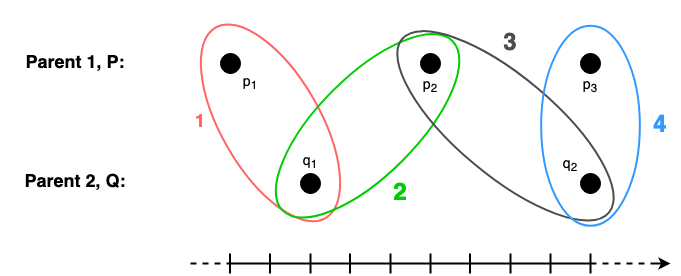
\includegraphics[width=.8\textwidth]{fig/uniform-crossover.png}
    \caption{A diagram showing multiple cases when calculating uniform crossover.}
    \label{fig:uniform-crossover}
\end{figure}

\subsubsection{Range tree}

A range tree is a binary tree. Each node contains information about the following:
\begin{itemize}
    \item An interval $[a,b]$ where $a \leq b$. 
    \item A minimum $min$ and maximum $max$ value. 
\end{itemize}
For a given node, this means that for $a \leq b \leq T$, the interval
$[y_a,y_b]$ has the minimum value $min$ and maximum value $max$. 

For each node where $a \neq b$, the left child has the interval $[a, \lfloor
(a+b)/2 \rfloor]$ and the right child has the interval $[\lceil
(a+b)/2 \rceil, b]$. The maximum and minimum of the node is the combined maximum
and minimum of the two children. For leaves, the range is a singleton range
$[c,c]$ and the minimum and maximum values are also the same. The minimum and
maximum values for each node is thus calculated recursively starting from the
leaves and moving up. 

Construction the range tree starts at the root. The root has the interval
$[0,T-1]$. The maximum and minimum values are the combination of the maximum and
minimum of the two children which is calculated recursively. The left child get
the index $[0, T/2]$ and the right child gets the index $[T/2 + 1, T]$. This
continues until the leaves where the minimum and maximum is set, resulting in
all the previous nodes now being updated with their minimum and maximum. 

\todo{Write about getting the min and max in a range}